\documentclass[Thesis.tex]{subfiles}
\begin{document}

\chapter{Surface panelization using periodic conformal maps}
\label{chp:periodic_conformal_maps}

This publication is joint work with Thilo R\"orig, Agata Kycia, and 
Moritz Fleischmann. It was previously published in~\cite{Roerig2014}.

\emph{Abstract:} 
We present a new method to obtain periodic conformal parameterizations of
surfaces with cylinder topology and describe applications to
architectural design and rationalization of surfaces. The method is
based on discrete conformal maps from the surface mesh to a cylinder or
cone of revolution. It comes with a number of degrees of freedom on
the boundary that can be used to obtain a variety of interesting
panelizations. We illustrate different choices of parameters for
\nurbs surface designs. Further, we describe how our parameterization
can be used to get a periodic boundary aligned hex-mesh on a
doubly-curved surface. We optimize this initial mesh to consist of a
limited number of planar regular hexagons that panel the surface.

\begin{figure}
  \centering
  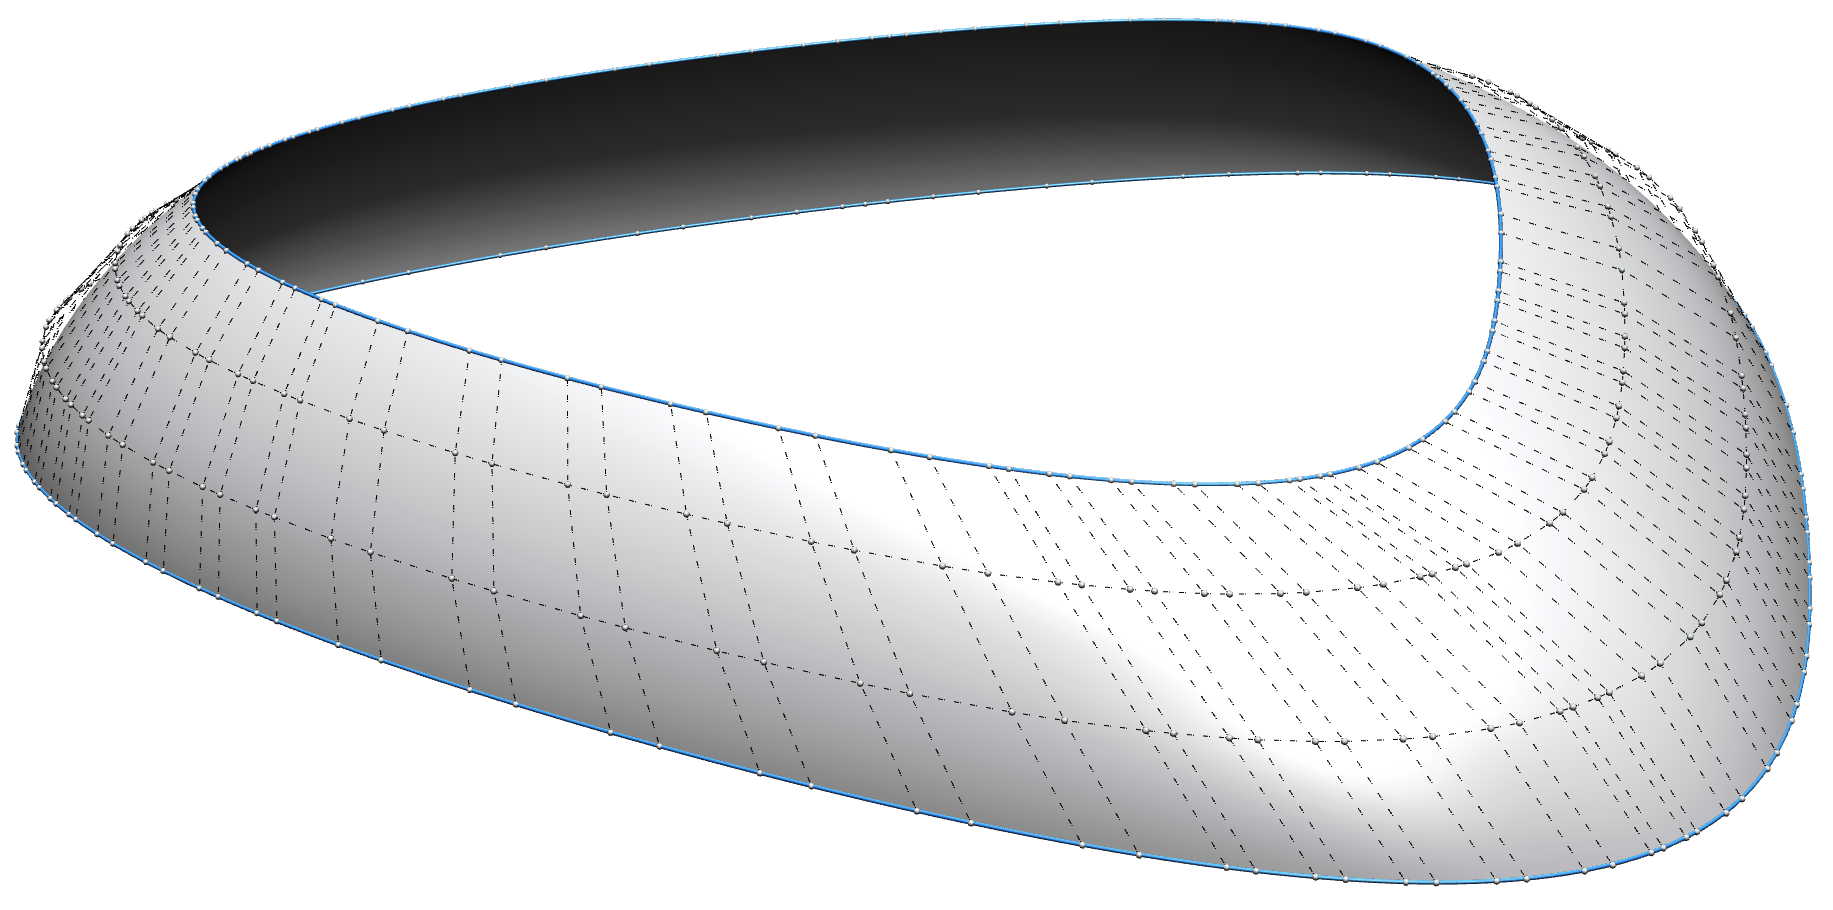
\includegraphics[width=0.49\textwidth]{images/teaser1_grid.png}
  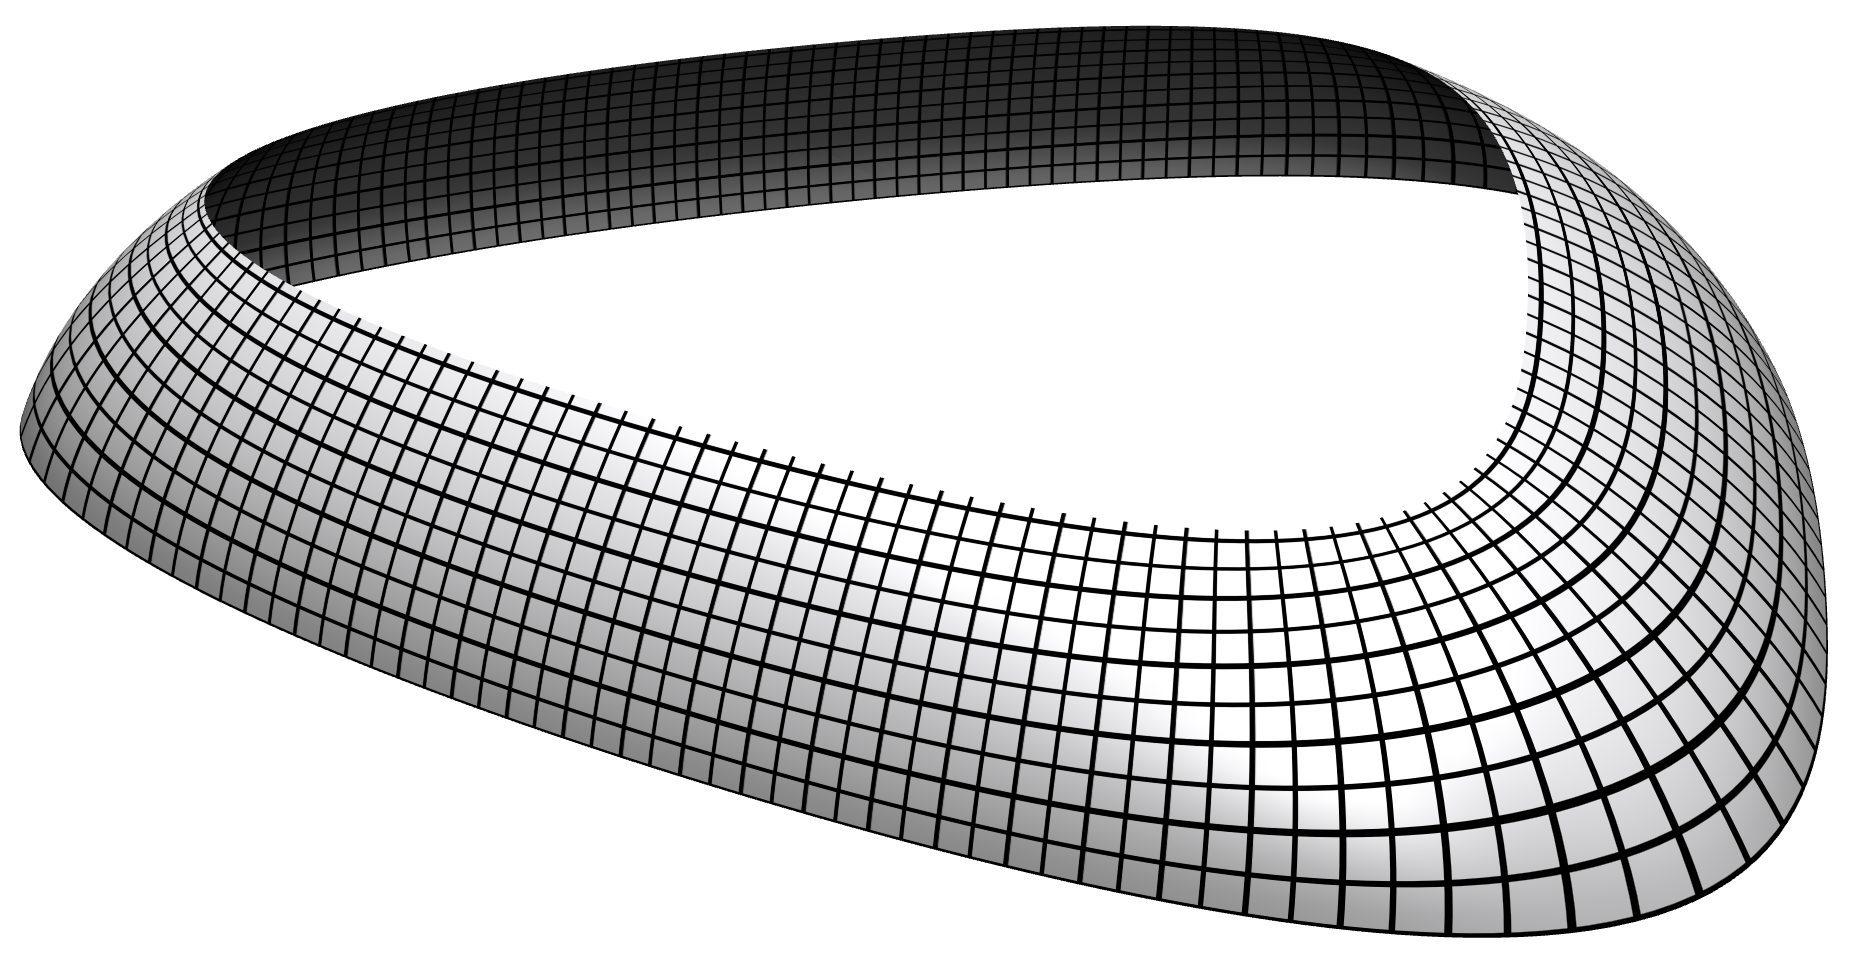
\includegraphics[width=0.49\textwidth]{images/teaser2_2.png}
  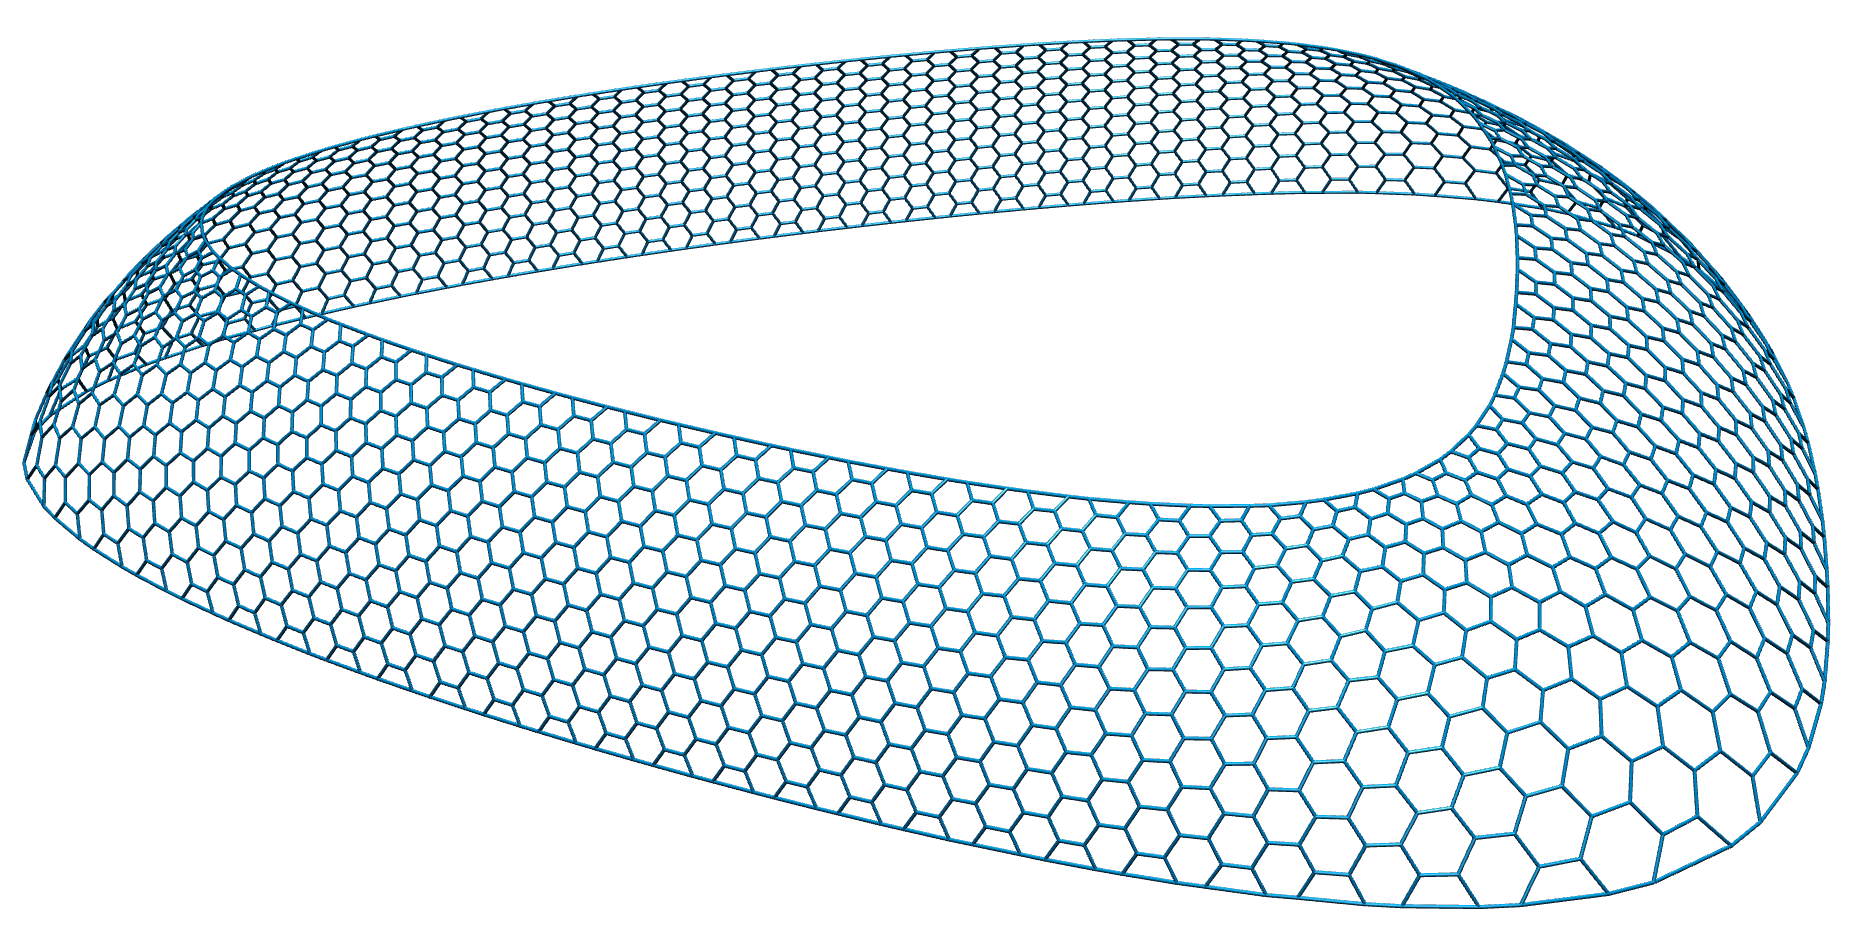
\includegraphics[width=0.49\textwidth]{images/teaser4_1.png}
  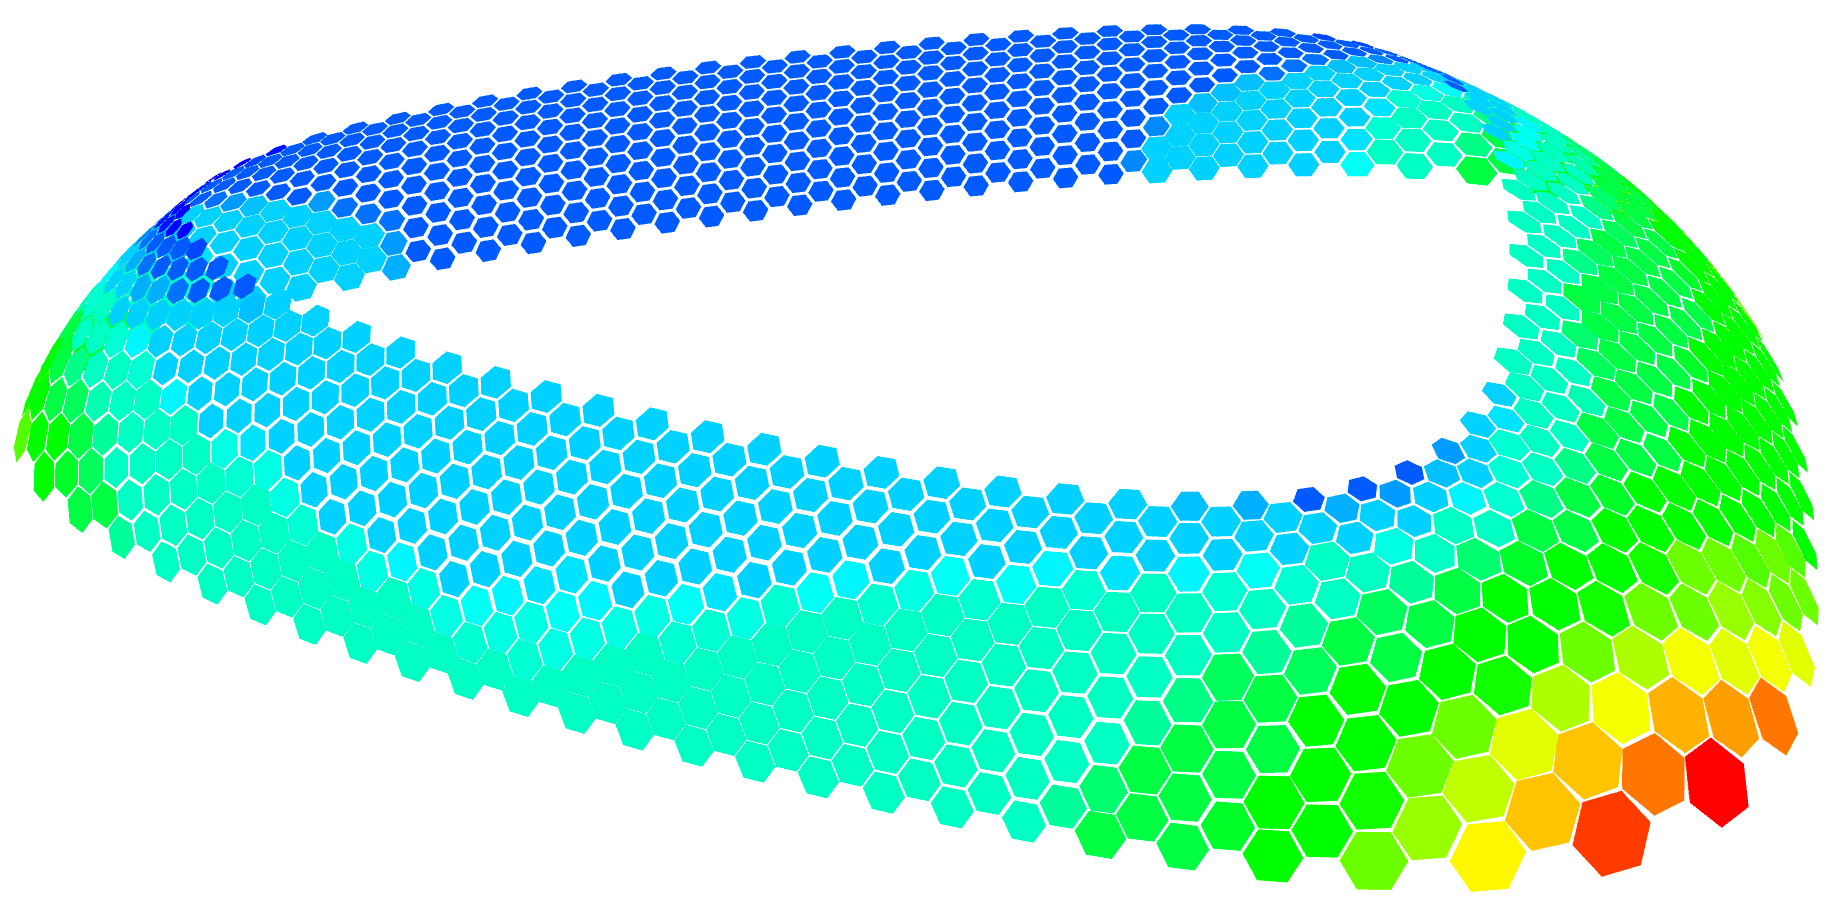
\includegraphics[width=0.49\textwidth]{images/teaser3.png}
  \caption{For a cylindrical \nurbs surface (top-left) we create a
    seamless periodic conformal parameterization (top-right). A new
    mesh (bottom-left) is then rationalized and the panels are
    optimized for quantized regular hexagons (bottom-right).}
  \label{fig:teaser}
\end{figure}

\def\subfilebibliography{}
\subfile{publications/AAG2014-Periodic/final/introduction.tex}
\subfile{publications/AAG2014-Periodic/final/parametrization.tex}
\subfile{publications/AAG2014-Periodic/final/conformal-parametrization.tex}
\subfile{publications/AAG2014-Periodic/final/boundary-conditions.tex}
\subfile{publications/AAG2014-Periodic/final/panelization.tex}
\subfile{publications/AAG2014-Periodic/final/hexagons.tex}
\subfile{publications/AAG2014-Periodic/final/implementation.tex}
\subfile{publications/AAG2014-Periodic/final/conclusion.tex}

\subfilebibliographytwo
\end{document}

%%% Local Variables:
%%% TeX-master: "Thesis.tex"
%%% End: